\documentclass{beamer}
\usepackage[utf8]{inputenc}
\usepackage{graphicx}
\usetheme{Ilmenau}

\title[Étape d'initialisation de gestion de projet]{Gestion de projets\\Le réseau PERT -- Le diagramme de Gantt}

\author{Ammar Inès -- Lecerf Geoffrey}
\institute{Université Montpellier II}
\date{11 octobre 2012}

\AtBeginSubsection[]{
	\begin{frame}<beamer>
	\frametitle{Plan}
	\tableofcontents[currentsection,currentsubsection]
	\end{frame}
}

\begin{document}

%%%%%% AFFICHE LA PAGE DE GARDE
\begin{frame}
\titlepage
\end{frame}

%%%%%% AFFICHE LE PLAN EN ENTIER
\begin{frame}{Plan}
\tableofcontents
\end{frame}

%%%%%% PARTIE I : PERT
\section{Le réseau PERT}
\subsection{Méthode PERT}
\begin{frame}{La méthode PERT}
	\begin{itemize}
		\item <+-| alert@+>\textbf{Program of Evaluation and Review Technic} : \\"Technique d'ordonnancement et de contrôle des programmes"
		\item <+-| alert@+>Représenter sous forme de graphe un \textbf{réseau} de \textbf{tâches} qui permet d'aboutir à la réalisation du projet
	\end{itemize}
\end{frame}

\subsection{Origines}
\begin{frame}{Origines}
	\textbf{Projet POLARIS(1957-1958)}\\
	\begin{itemize}
		\pause \item  <+-|alert@+>Ingénieurs de la marine américaine mettent en place une méthode de travail pour coordonner les tâches des entreprises impliquées dans ce projet
		\item <+-|alert@+>Réduction de 7 à 14 ans de la durée du projet
	\end{itemize}
\end{frame}

\subsection{Notion de réseau}
\begin{frame}{Qu'est-ce qu'un réseau ?}
	Ensemble d'éléments reliés entre eux, représenté sous forme de graphe.
	\begin{figure}
		\pause \includegraphics[width=6.5cm, height=5cm]{PERT/reseau1.png}
	\end{figure}
\end{frame}

\begin{frame}{Le réseau Internet}
	\begin{figure}
		\includegraphics[width=0.8\textwidth, height=0.8\textheight]{PERT/reseauI.png}
	\end{figure}
\end{frame}

\begin{frame}{Pourquoi parle-t-on de réseau PERT ?}
	Consiste à décomposer de façon \textbf{chronologique}, sous forme de réseau, un projet en plusieurs \textbf{étapes} reliées par des \textbf{tâches} à effectuer.
\end{frame}

\begin{frame}{Exemple de réseau PERT}
	\begin{figure}
		\includegraphics[width=0.8\textwidth, height=0.8\textheight]{PERT/reseau.png}
	\end{figure}
\end{frame}

\subsection{Tableau des tâches}
\begin{frame}{Le tableau des tâches}
Répertorier dans un tableau :
	\begin{itemize}
		\item <+-|alert@+>les différentes tâches 
		\item <+-|alert@+>la durée des tâches
		\item <+-|alert@+>les tâches antécédentes à la tâche considérée
	\end{itemize}
\end{frame}

\begin{frame}{Tableau des tâches}
	\begin{figure}
		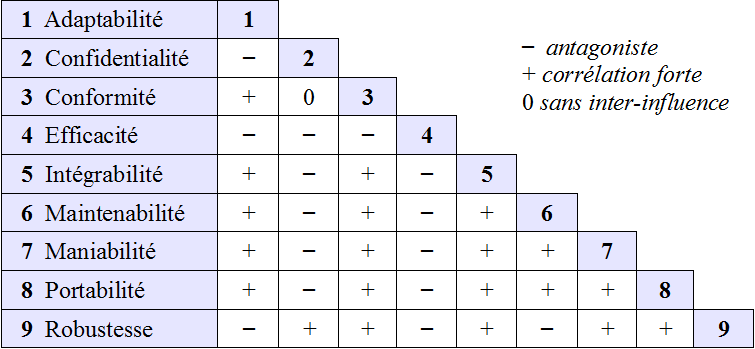
\includegraphics[width=\textwidth, height=0.7\textheight]{PERT/tableau.png}
	\end{figure}
\end{frame}

\subsection{Réalisation du graphe}
\begin{frame}{Présentation}
	\begin{itemize}
		\item <+-|alert@+>\textbf{Tâche} : déroulement dans le temps d'une opération en spécifiant l'action à effectuer ainsi que le temps pour la réaliser
		\begin{figure}
			\pause \includegraphics[width=3cm, height=1cm]{PERT/fleche.png}
		\end{figure}
		\pause \item <+-|alert@+>\textbf{Etape} : commencement et fin d'une tâche
		\begin{figure}
			\pause \includegraphics[width=2cm, height=2cm]{PERT/cercle.png}
		\end{figure}
	\end{itemize}
\end{frame}

\begin{frame}{Les différentes tâches}
	\begin{itemize}
		\item <+-|alert@+>\textbf{succesives} : tâches qui se suivent dans le temps
		\pause \includegraphics[width=0.8\textwidth, height=0.25\textheight]{PERT/success.png}
	\end{itemize}
\end{frame}

\begin{frame}{Les différentes tâches}
	\begin{itemize}
		\item <+-|alert@+>\textbf{simultanées} : tâches s'effectuant en même temps
		\pause \includegraphics[width=0.8\textwidth, height=0.8\textheight]{PERT/simult.png}
	\end{itemize}
\end{frame}

\begin{frame}{Les différentes tâches}
	\begin{itemize}
		\item <+-|alert@+>\textbf{convergentes} : tâches nécessaires à l'effectuation d'une tâche postérieure 
		\pause \includegraphics[width=0.8\textwidth, height=0.7\textheight]{PERT/conv.png}
	\end{itemize}
\end{frame}

\begin{frame}{Construction du diagramme}
	\begin{itemize}
		\item<+-|alert@+>\textbf{Tâche} : flèche reliant 2 étapes. On indique son nom et durée.
		\item<+-|alert@+>\textbf{Etape} : 
			\begin{enumerate}
				\item <+-|alert@+>\textit{numéro étape}
				\item <+-|alert@+>\textit{date au plus tôt} : date à laquelle la tâche pourra être commencée au plus tôt
				\item <+-|alert@+>\textit{date au plus tard} : date à laquelle la tâche doit être terminée à tout prix
			\end{enumerate}
	\end{itemize}
\end{frame}

\begin{frame}{Date au plus tôt}
	\begin{figure}
		\includegraphics[width=0.8\textwidth, height=0.8\textheight]{PERT/datedebut.png}
	\end{figure}
\end{frame}

\begin{frame}{Date au plus tard}
	\begin{figure}
		\includegraphics[width=0.8\textwidth, height=0.8\textheight]{PERT/datefin.png}
	\end{figure}
\end{frame}

\begin{frame}{Exemple de réseau PERT terminé}
	\begin{figure}
		\includegraphics[width=\textwidth, height=0.65\textheight]{PERT/diag.png}
	\end{figure}
\end{frame}

\begin{frame}{Chemin critique}
Chemin qui donne le temps le plus long sur le diagramme.\\
Tout retard sur ce chemin engendrera nécessairement un retard de l'achèvement du projet.
\end{frame}

\begin{frame}{Chemin critique du réseau PERT}
	\begin{figure}
		\includegraphics[width=\textwidth, height=0.65\textheight]{PERT/chemin.png}
	\end{figure}
\end{frame}


%%%%%% PARTIE II : GANTT
\section{Le diagramme de Gantt}
\subsection{Présentation-Historique}
\begin{frame}{Présentation-Historique}
	\begin{itemize}
		\item <+-|alert@+>Conçu en 1917 par Henry Gantt pour améliorer la gestion de certains ateliers d'entreprises
		\item <+-|alert@+>Le diagramme de Gantt est un outil qui permet de modéliser la planification de tâches nécessaires à la réalisation d'un projet. Il est très utile pour tout projet.
		\item <+-|alert@+>Un moyen de communication entre les différents acteurs du projet.
	\end{itemize}
\end{frame}

\subsection{Intérêts}
\begin{frame}{Pourquoi utiliser le diagramme de Gantt }
	\begin{itemize}
		\item <+-|alert@+>Adaptable à tous, utilisable pour tous les domaines
		\item <+-|alert@+>Structure les pensées (ordonner les tâches...)
		\item <+-|alert@+>Permet de bien suivre la progression du projet et améliore l'organisation du travail
		\item <+-|alert@+>Se planifie et permet de visualiser plus facilement la durée totale du projet
		\item <+-|alert@+>Dynamique : en cas de modification, il recalcule automatiquement les dates et durées de chaque tâche
	\end{itemize}
\end{frame}

\subsection{Réalisation du diagramme}
\begin{frame}{Réalisation du diagramme }
	\begin{itemize}
		\item<+-|alert@+>Liste les tâches qui devront être accomplies, chaque tâche doit avoir des limites chronologiques bien définies (durée) et doit être associée à un responsable (ressources)
			\begin{itemize}
				\item<+-|alert@+>\textbf{durée d'une tâche} : attribuer une date de début, une date de fin pour chaque tâche
				\item<+-|alert@+>\textbf{attribution des ressources} : une ou plusieurs personnes sont amenées à effectuer chaque tâche, souvent représentées en pourcentage (100\% correspond à une personne consacrée à plein temps à la tâche, 300\% à 3 personnes...)
			\end{itemize}
	\end{itemize}
\end{frame}

\begin{frame}{Réalisation du diagramme }
	\begin{itemize}
		\item<+-|alert@+>\textbf{Agencement et synchronisation des tâches} : \\
		Les tâches d'un projet peuvent s'agencer de façons différentes. Chaque tâche est reliée à une autre selon un processus différent en fonction des contraintes d'exécution du projet.
	\end{itemize}
\end{frame}

\begin{frame}{Réalisation du diagramme}
On distingue 4 types de liaison :
	\begin{itemize}
		\item<+-|alert@+>\textbf{Fin-Début} : la fin d'une tâche coïncide avec le démarrage d'une autre
			\begin{figure}
				\pause 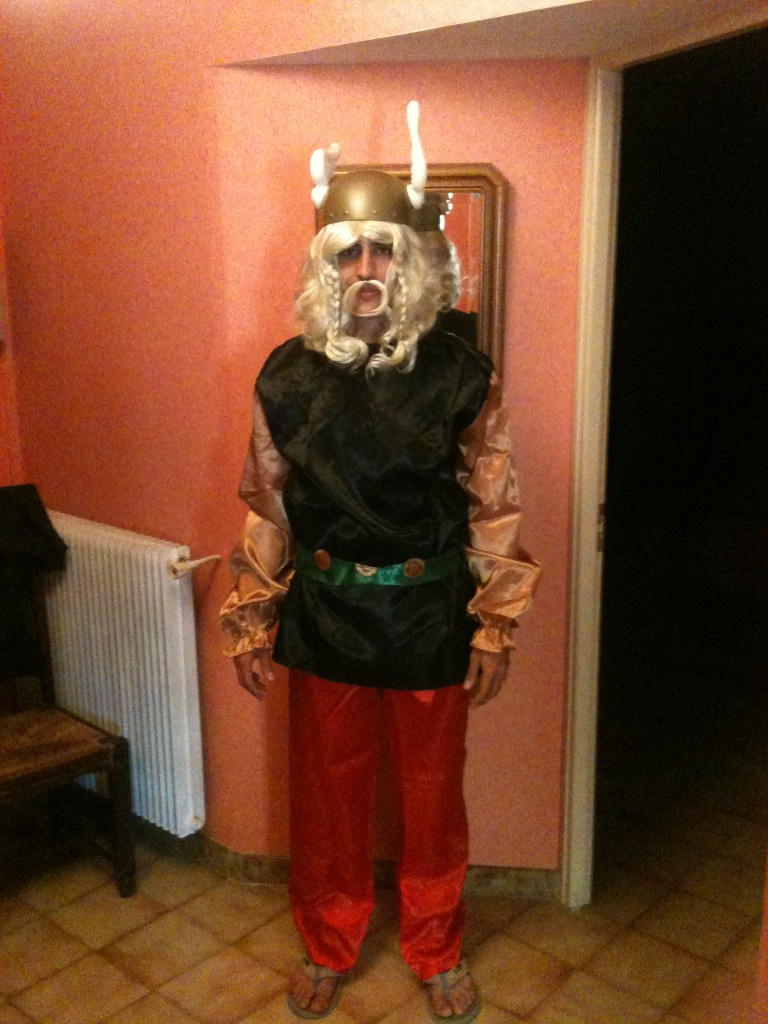
\includegraphics[width=0.25\textwidth, height=0.25\textheight]{GANTT/1.png}
			\end{figure}
		\pause \item<+-|alert@+>\textbf{Fin-Fin} : le cas où 2 (ou plusieurs) tâches doivent se terminer en même temps
			\begin{figure}
				\pause 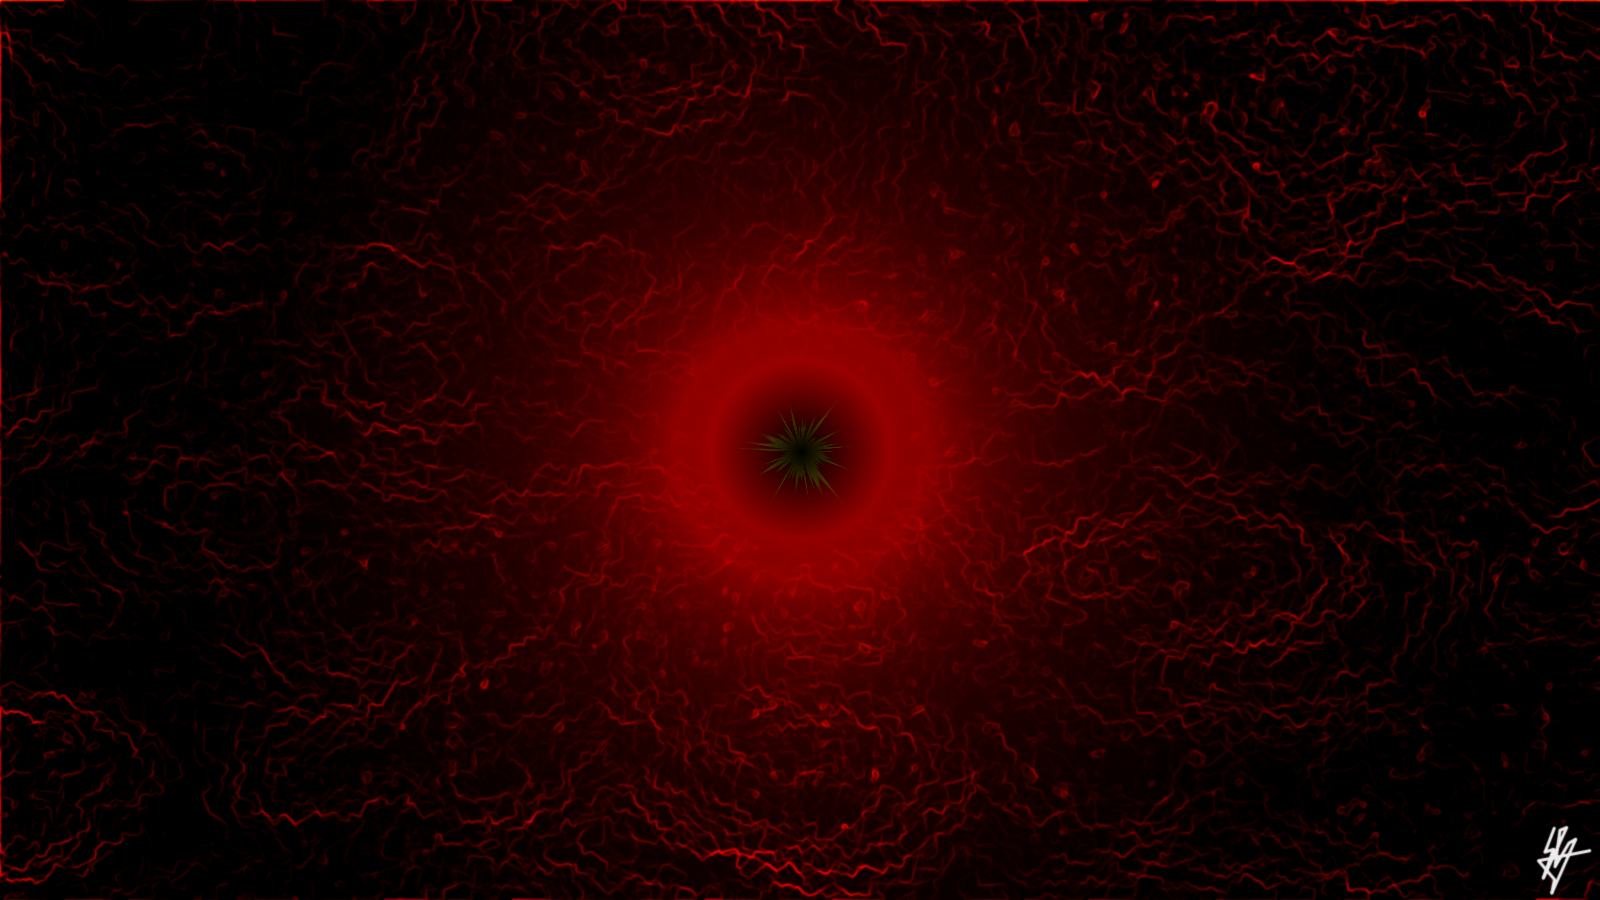
\includegraphics[width=0.25\textwidth, height=0.25\textheight]{GANTT/2.png}
			\end{figure}
	\end{itemize}
\end{frame}

\begin{frame}{Réalisation du diagramme}
	\begin{itemize}
		\item<+-|alert@+>\textbf{Début-Fin} : la fin d'une tâche est calculée par rapport au début d'une autre
			\begin{figure}
				\pause 
\includegraphics[width=0.25\textwidth, height=0.25\textheight]{GANTT/3.png}
			\end{figure}
		\pause \item<+-|alert@+>\textbf{Début-Début} : le démarrage d'une ou plusieurs tâches s'effectue en même temps
			\begin{figure}
				\pause 
\includegraphics[width=0.25\textwidth, height=0.25\textheight]{GANTT/4.png}
			\end{figure}
	\end{itemize}
\end{frame}

\begin{frame}{Exemple simple de diagramme Gantt}
L'exemple ci-dessous effectué à l'aide du logiciel GANTT PROJECT.\\
On trouve la liaison Fin-Début pour les trois tâches T1, T2 et T3.
	\begin{figure}
		\includegraphics[width=\textwidth, height=0.24\textheight]{GANTT/5.png}
	\end{figure}
Les tâches sont représentées sous forme d'un rectangle d'une longueur proportionnelle à leur durée.
\end{frame}

\begin{frame}{Exemple simple de diagramme Gantt}
Le tableau correspondant à cet exemple 
	\begin{figure}
		\pause \includegraphics[width=\textwidth, height=0.3\textheight]{GANTT/7.png}
	\end{figure}
\end{frame}

\begin{frame}{Chemin critique}
Un chemin critique est l'ensemble des tâches critiques qui donnent le temps le plus long du projet.\\ 
Tout retard sur l'une de ces tâches entraînera un retard de l'achèvement du projet.
	\begin{figure}
		\pause 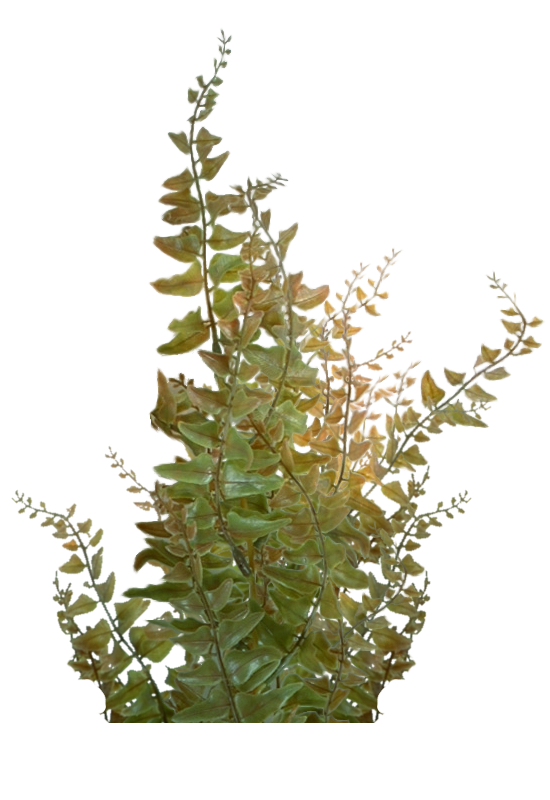
\includegraphics[width=\textwidth, height=0.24\textheight]{GANTT/6.png}
	\end{figure}
\end{frame}

\subsection{Les différents logiciels de Gantt}
\begin{frame}{Les différents logiciels de Gantt}
Plusieurs logiciels de planification sont disponibles, certains sont gratuits mais offrent des possibilités limitées, d'autres sont payants mais plus complets et puissants.\\
On retrouve essentiellement:
	\begin{itemize}
		\pause \item <+-|alert@+>Microsoft Excel
		\item <+-|alert@+>PowerPoint
		\item <+-|alert@+>GanttProject
		\item <+-|alert@+>ProjectPro
		\item <+-|alert@+>Gantter
		\item <+-|alert@+>Asta Powerproject
		\item <+-|alert@+>Microsoft Project
	\end{itemize}
\end{frame}


\end{document}
